% !TEX root = ../main.tex

\chapter{Ejemplos de uso}
\label{ch:otro}

En esta sección se presentan diversos casos prácticos que ilustran el funcionamiento de la herramienta \textit{QuadFix} en diferentes contextos. Se ha estructurado la sección en tres categorías según la proporción del objeto rectificado: cuadrados, folios (con proporción $\sqrt{2}:1$) y otras proporciones personalizadas.


\section{Rectificación de Cuadrados}

A continuación, se presentan dos ejemplos representativos de rectificación de superficies cuadradas, en los que se demuestra cómo la herramienta \textit{QuadFix} transforma correctamente imágenes distorsionadas en representaciones frontales y proporcionales.

\subsection*{Ejemplo 1: Tablero de juego}

En la Figura~\ref{fg:tablero-original}, se muestra la imagen original de un tablero de juego tomada en perspectiva. El usuario ha seleccionado manualmente las esquinas del cuadrado, y ha establecido la razón de aspecto como $1:1$.

La Figura~\ref{fg:tablero-rectificado} presenta el resultado tras aplicar la transformación proyectiva. Se observa cómo la imagen del tablero ha sido rectificada adecuadamente, restaurando su forma cuadrada. Además, los elementos visuales situados a la derecha del tablero también han sido transformados coherentemente, como resultado de la aplicación de la homografía.

En la Figura~\ref{fg:tablero-descarga}, se muestra el mensaje de confirmación que indica que la descarga de la imagen se ha realizado correctamente, ofreciendo así una retroalimentación visual positiva al usuario.

\begin{figure}[H]
    \centering
    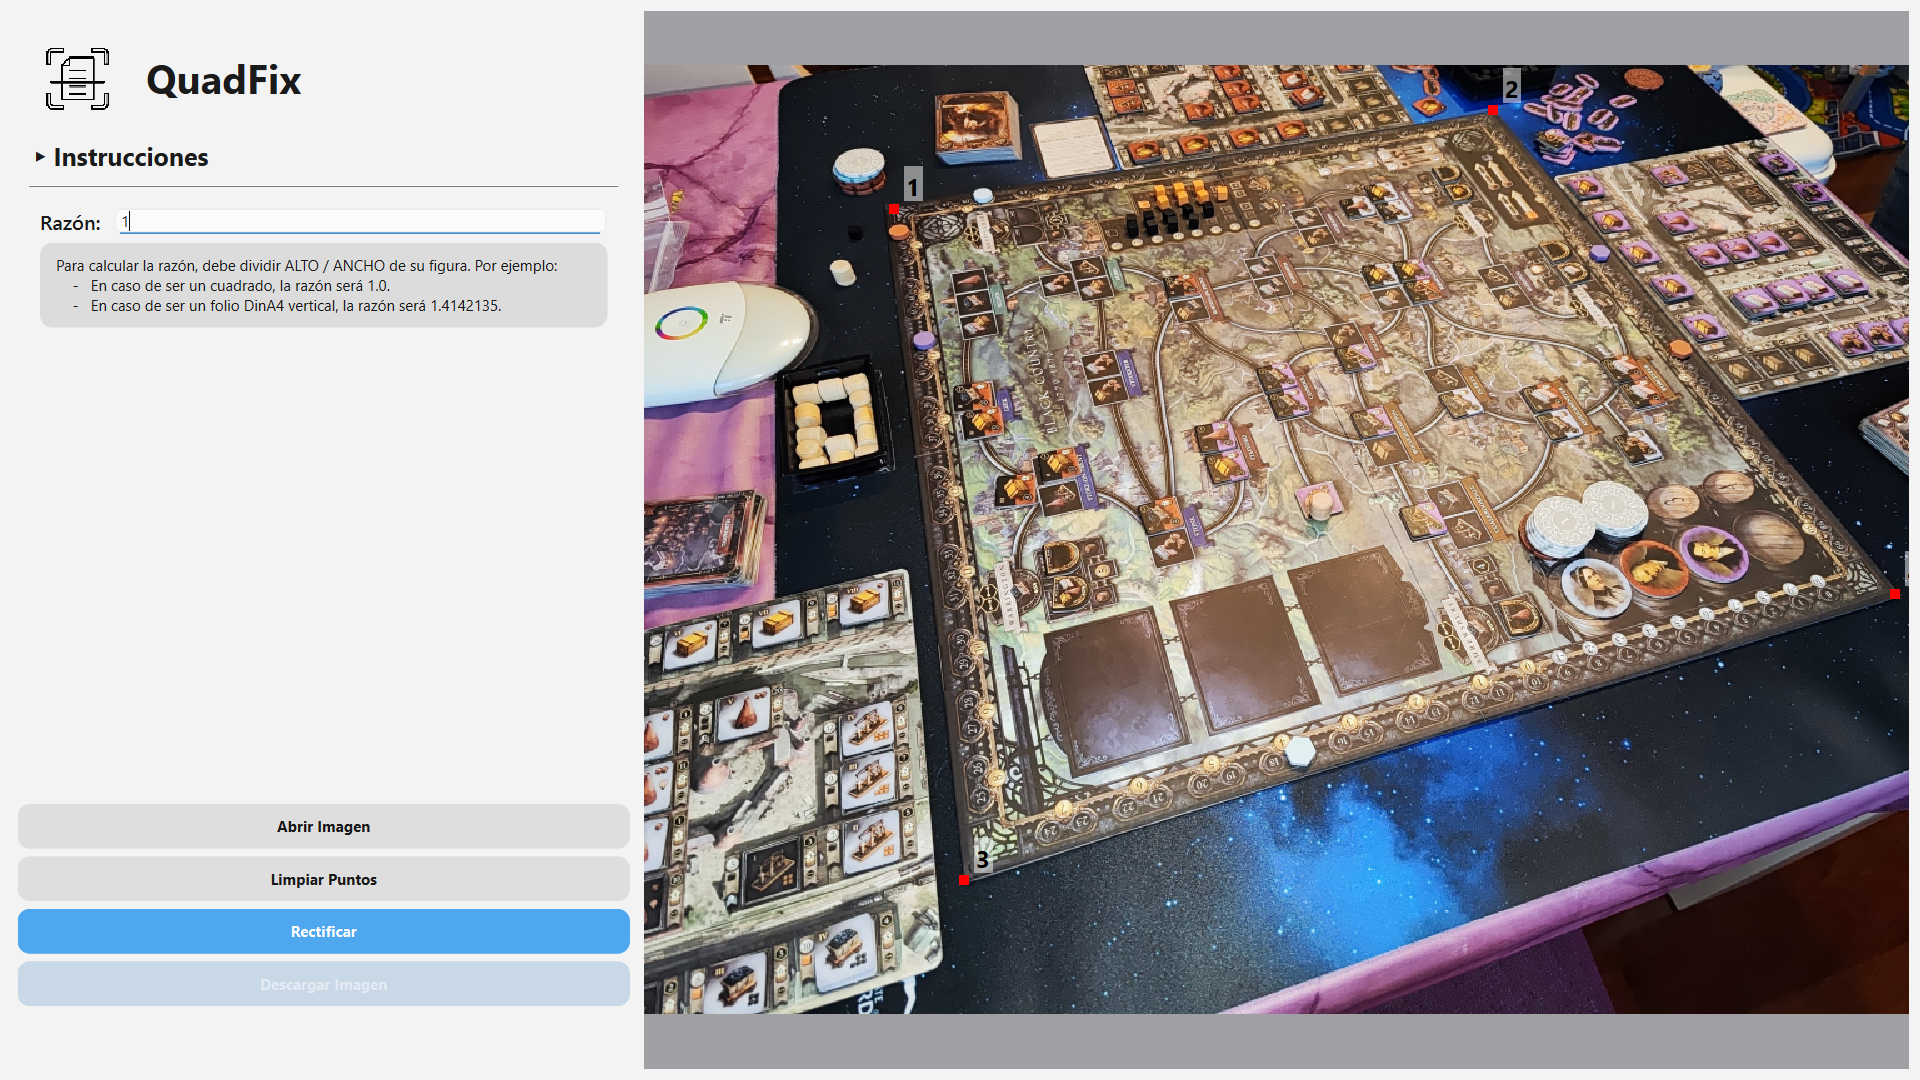
\includegraphics[width=0.70\textwidth]{figures/4.Examples/Cuadrado/Juego1.png}
    \caption{Imagen original del tablero de juego con esquinas marcadas y razón $1:1$}
    \label{fg:tablero-original}
\end{figure}

\begin{figure}[H]
    \centering
    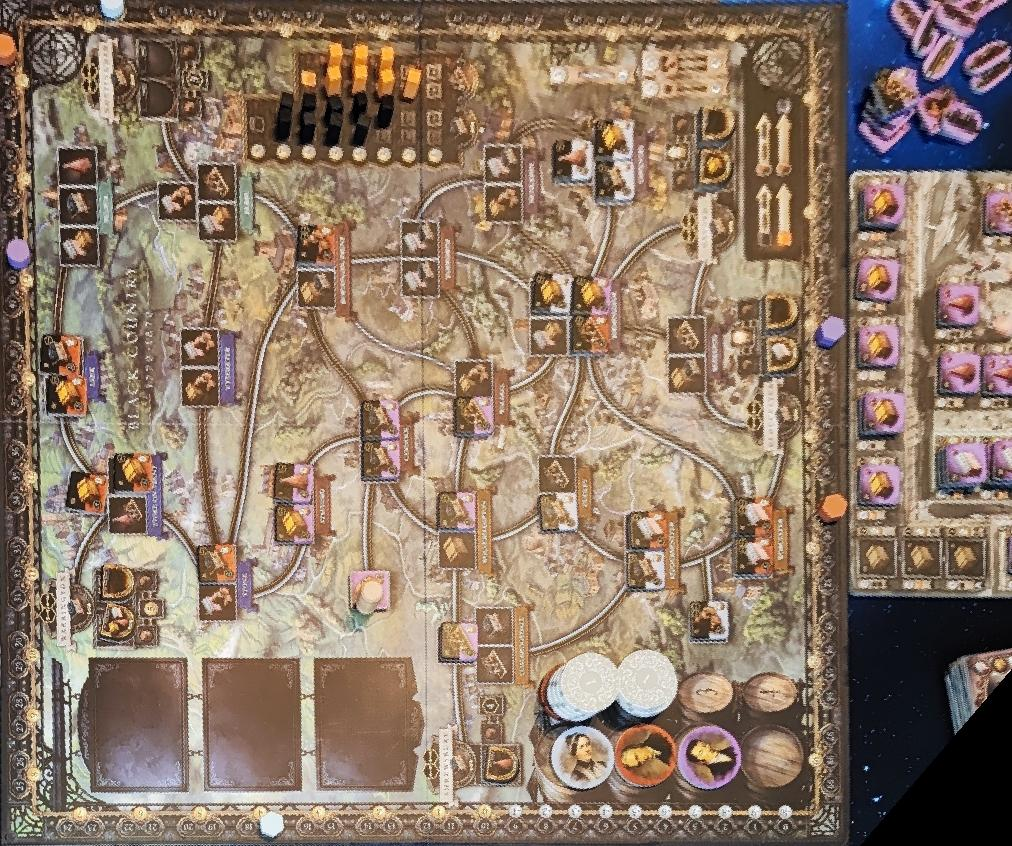
\includegraphics[width=0.50\textwidth]{figures/4.Examples/Cuadrado/Juego2.jpeg}
    \caption{Imagen rectificada del tablero de juego}
    \label{fg:tablero-rectificado}
\end{figure}

\begin{figure}[H]
    \centering
    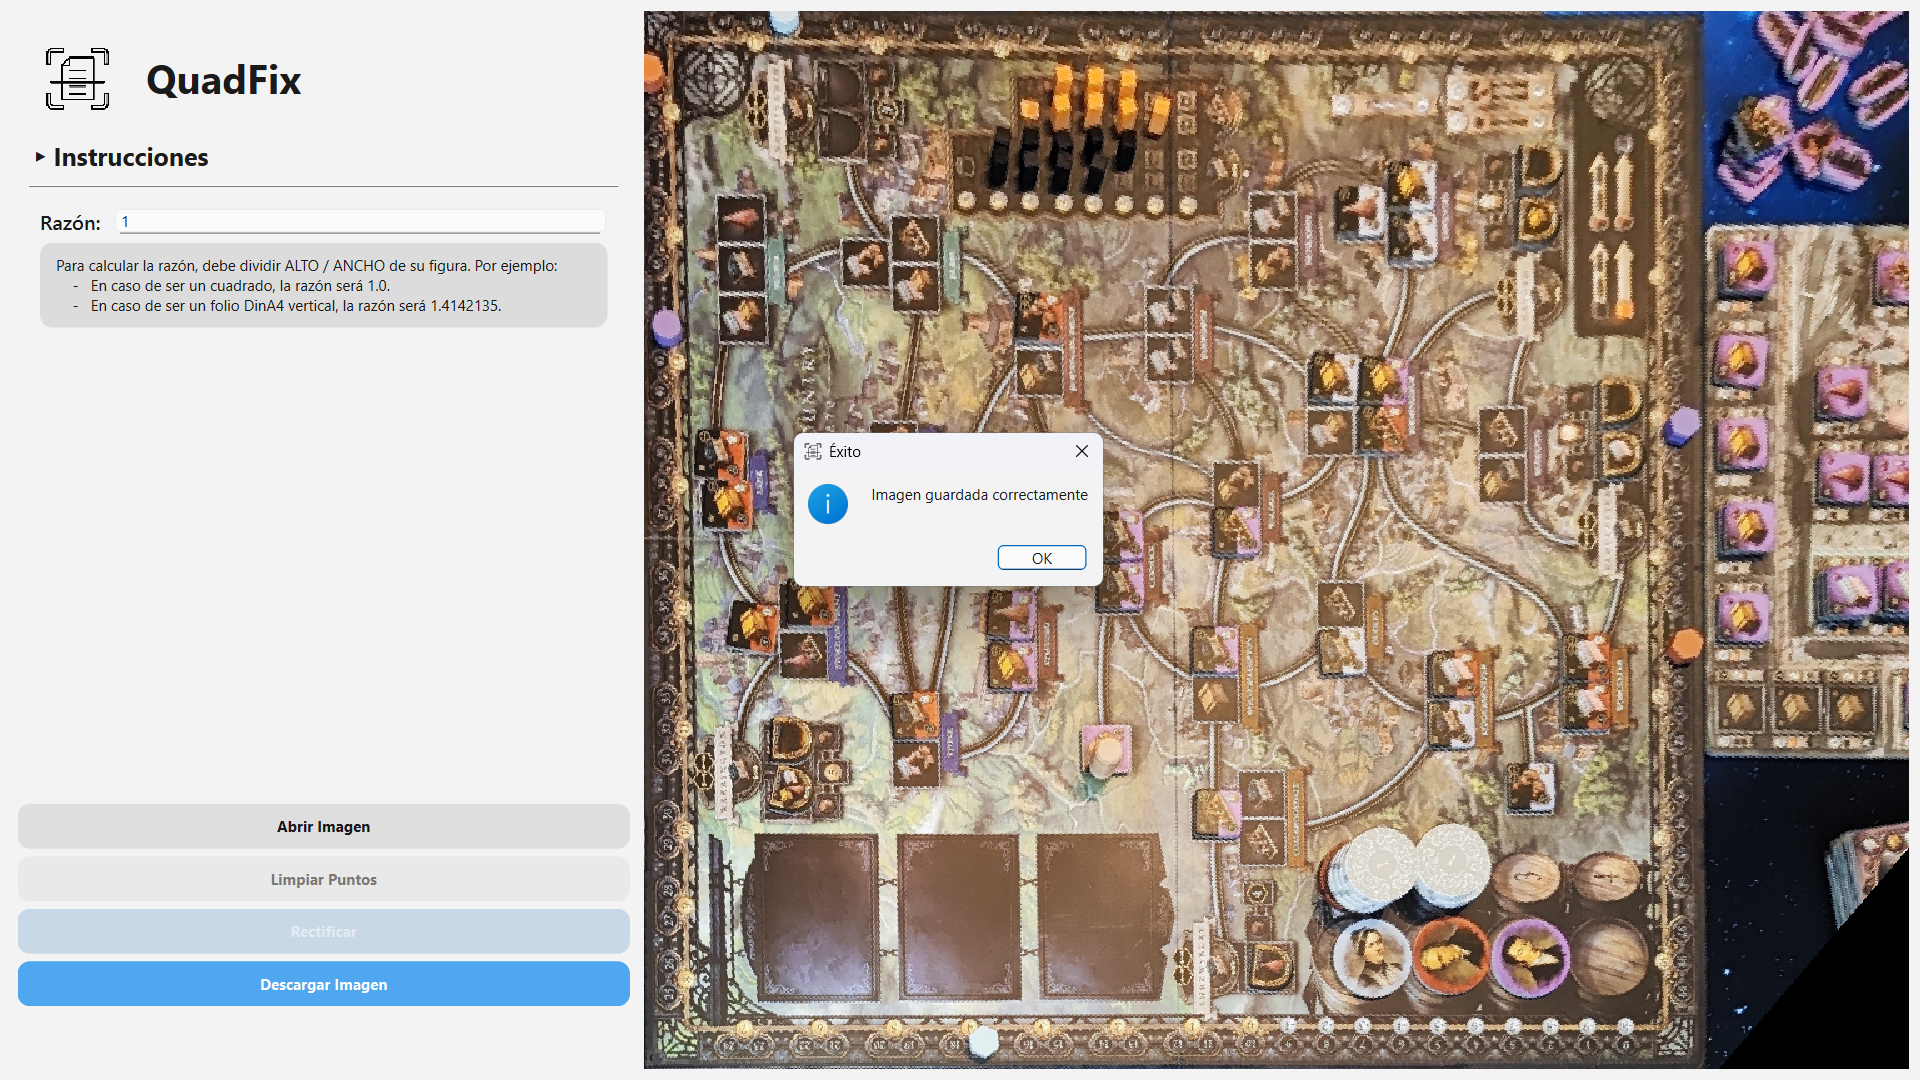
\includegraphics[width=0.70\textwidth]{figures/4.Examples/Cuadrado/Juego3.png}
    \caption{Mensaje de éxito tras la descarga de la imagen rectificada}
    \label{fg:tablero-descarga}
\end{figure}


\subsection*{Ejemplo 2: Vinilo decorativo}

La Figura~\ref{fg:vinilo-original} muestra una imagen de un vinilo cuadrado adherido a una superficie, tomada en perspectiva oblicua. Junto al vinilo se encuentra un objeto que ayuda a apreciar la distorsión geométrica presente en la toma.

\begin{figure}[H]
    \centering
    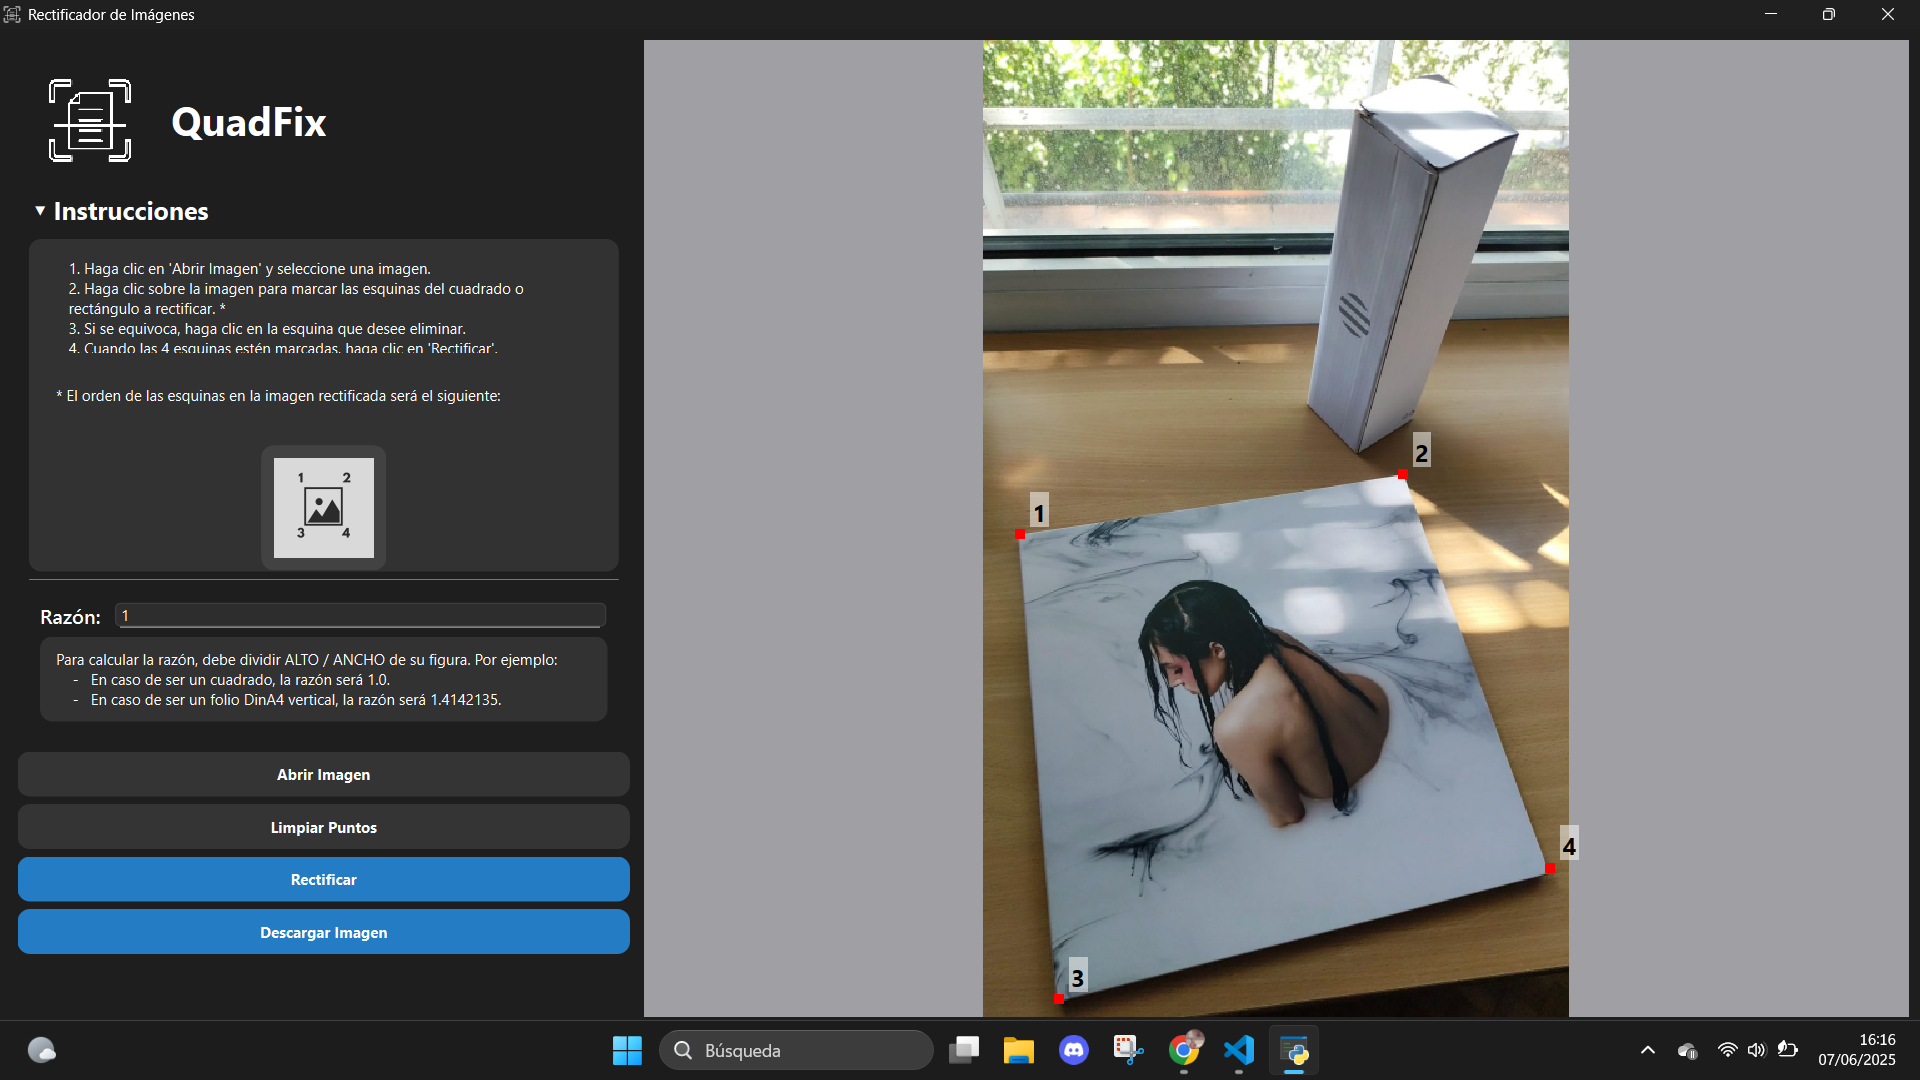
\includegraphics[width=0.85\textwidth]{figures/4.Examples/Cuadrado/Vinilo1.png}
    \caption{Imagen original de un vinilo con perspectiva oblicua}
    \label{fg:vinilo-original}
\end{figure}

Tras seleccionar las esquinas y establecer la razón de aspecto como $1:1$, se aplica la rectificación. El resultado puede apreciarse en la Figura~\ref{fg:vinilo-rectificado}, donde se observa cómo el vinilo ha recuperado su forma cuadrada original, sin las distorsiones previas.

\begin{figure}[H]
    \centering
    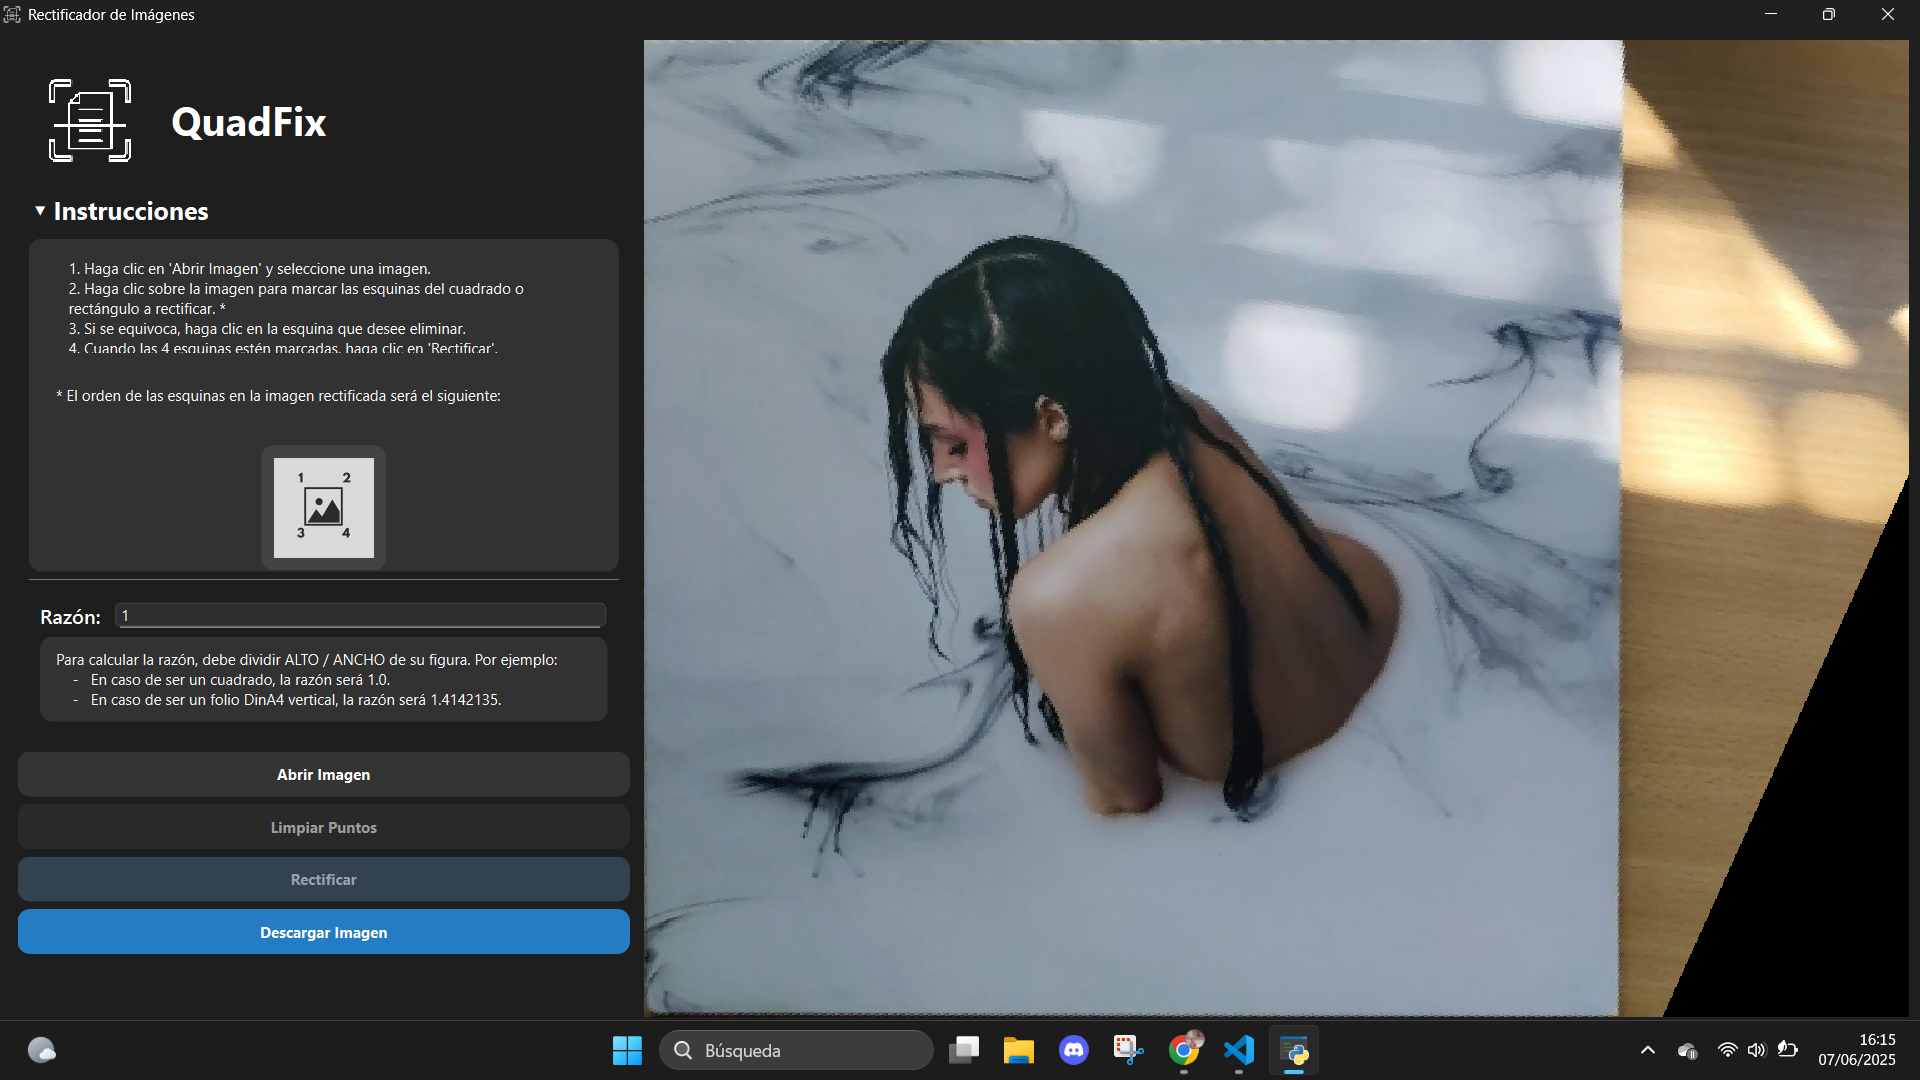
\includegraphics[width=0.85\textwidth]{figures/4.Examples/Cuadrado/Vinilo2.png}
    \caption{Imagen rectificada del vinilo, mostrada en la aplicación}
    \label{fg:vinilo-rectificado}
\end{figure}




\section{Rectificación de Folios}

En esta sección se muestra la rectificación de imágenes de folios, cuya proporción aproximada es $\sqrt{2}:1$. Dado que la interfaz de \textit{QuadFix} no admite expresiones simbólicas, el usuario introduce manualmente el valor numérico $1.4142$ como razón de aspecto.

En la Figura~\ref{fg:folio-original} se presenta una imagen de entrada correspondiente a un folio fotografiado con perspectiva. El usuario ha seleccionado manualmente las cuatro esquinas y ha introducido la razón mencionada anteriormente. La Figura~\ref{fg:folio-rectificado} muestra el resultado tras la rectificación proyectiva. Se observa cómo el documento recupera su forma rectangular con proporción adecuada, obteniéndose una visualización similar a una vista cenital.

\begin{figure}[H]
    \centering
    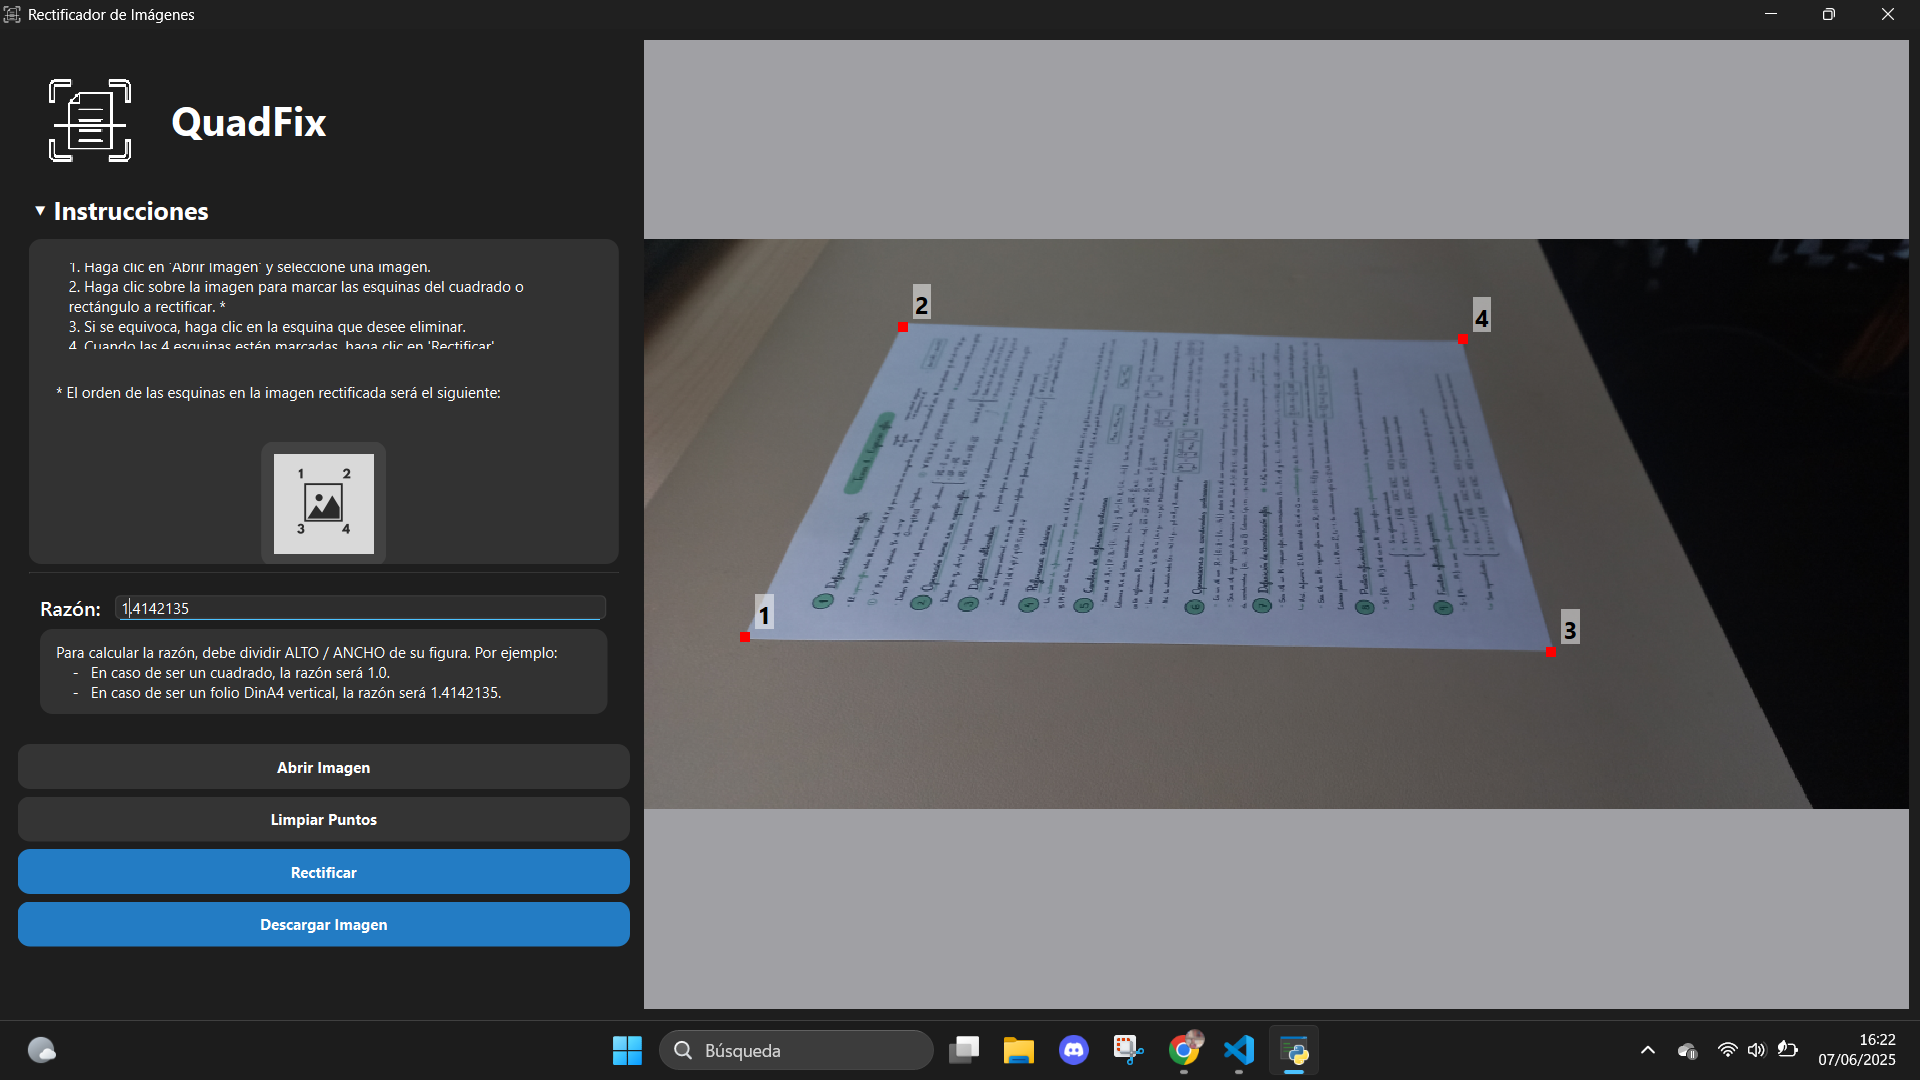
\includegraphics[width=0.75\textwidth]{figures/4.Examples/A4/Example1.png}
    \caption{Folio con perspectiva y esquinas seleccionadas. Razón introducida: 1.4142}
    \label{fg:folio-original}
\end{figure}

\begin{figure}[H]
    \centering
    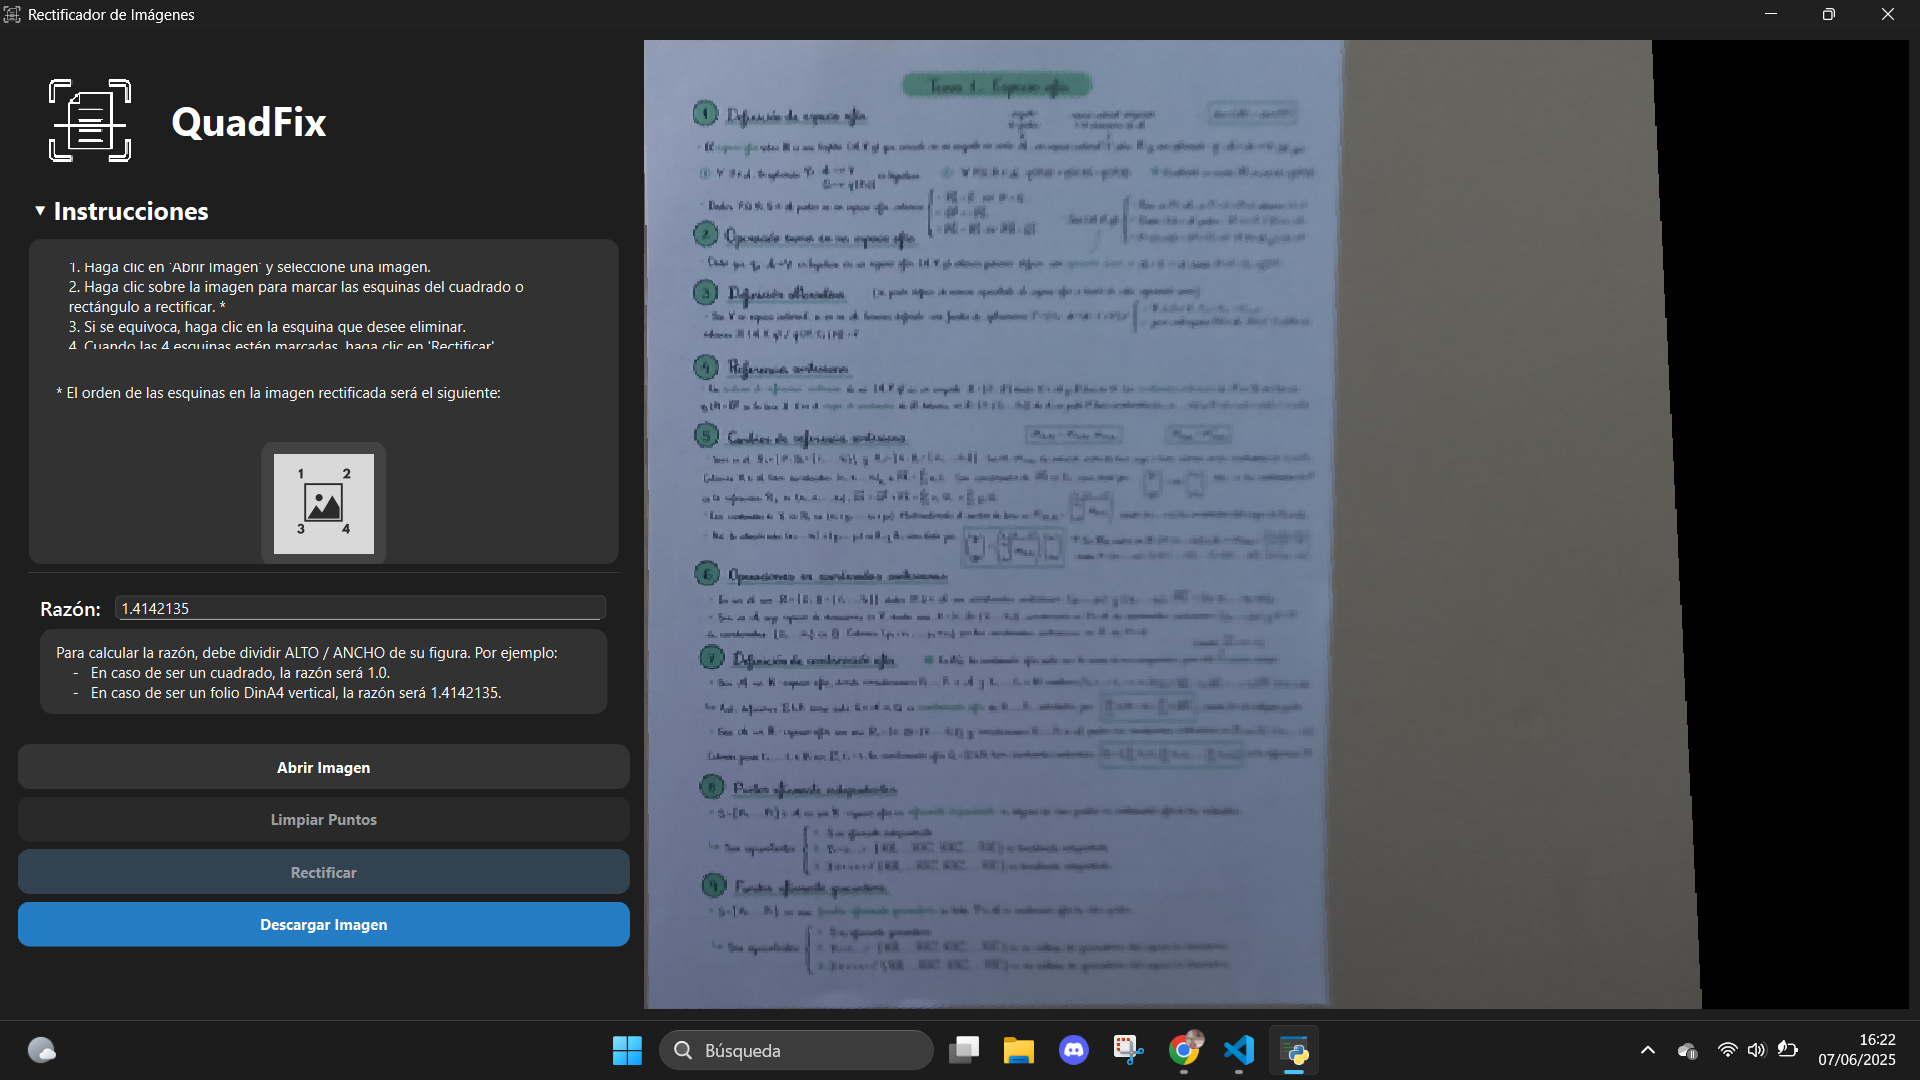
\includegraphics[width=0.75\textwidth]{figures/4.Examples/A4/Example2.png}
    \caption{Folio rectificado}
    \label{fg:folio-rectificado}
\end{figure}

Finalmente, en la Figura~\ref{fg:folios-multiples} se recogen cuatro ejemplos adicionales de imágenes de folios tomadas desde diferentes ángulos. Cada fotografía original aparece acompañada por una flecha que indica su transformación mediante \textit{QuadFix}. A pesar de que la rectificación es correcta desde el punto de vista geométrico, puede apreciarse que la calidad visual de las imágenes transformadas es limitada. Esta cuestión se discute con más detalle en el apartado de Limitaciones Actuales (ver Sección~\ref{sec:limitaciones}).

\begin{figure}[H]
    \centering
    \includegraphics[width=0.73\textwidth]{figures/4.Examples/A4/Examples.png}
    \caption{Ejemplos de folios en distintas perspectivas y sus correspondientes rectificaciones}
    \label{fg:folios-multiples}
\end{figure}


\subsection{Otras proporciones}

Además de cuadrados y formatos estandarizados como el DIN A4, la herramienta \textit{QuadFix} permite rectificar objetos con proporciones arbitrarias especificadas por el usuario. A continuación se presentan dos ejemplos representativos: un libro con formato personalizado y un caso particular donde la interpretación de la proporción puede llevar a errores si no se ajusta adecuadamente la orientación de entrada.

\subsubsection*{Ejemplo 1: Libro de Topología}

En este caso se utiliza como imagen de entrada la portada de un libro con dimensiones conocidas: $24$ cm de alto por $17.2$ cm de ancho. Esto corresponde a una razón de aspecto de aproximadamente $1.395$ (alto/ancho), que el usuario debe introducir manualmente en la interfaz.

La Figura~\ref{fg:libro-original} muestra la imagen dentro de la aplicación, con las esquinas marcadas y la proporción introducida por el usuario.

\begin{figure}[H]
    \centering
    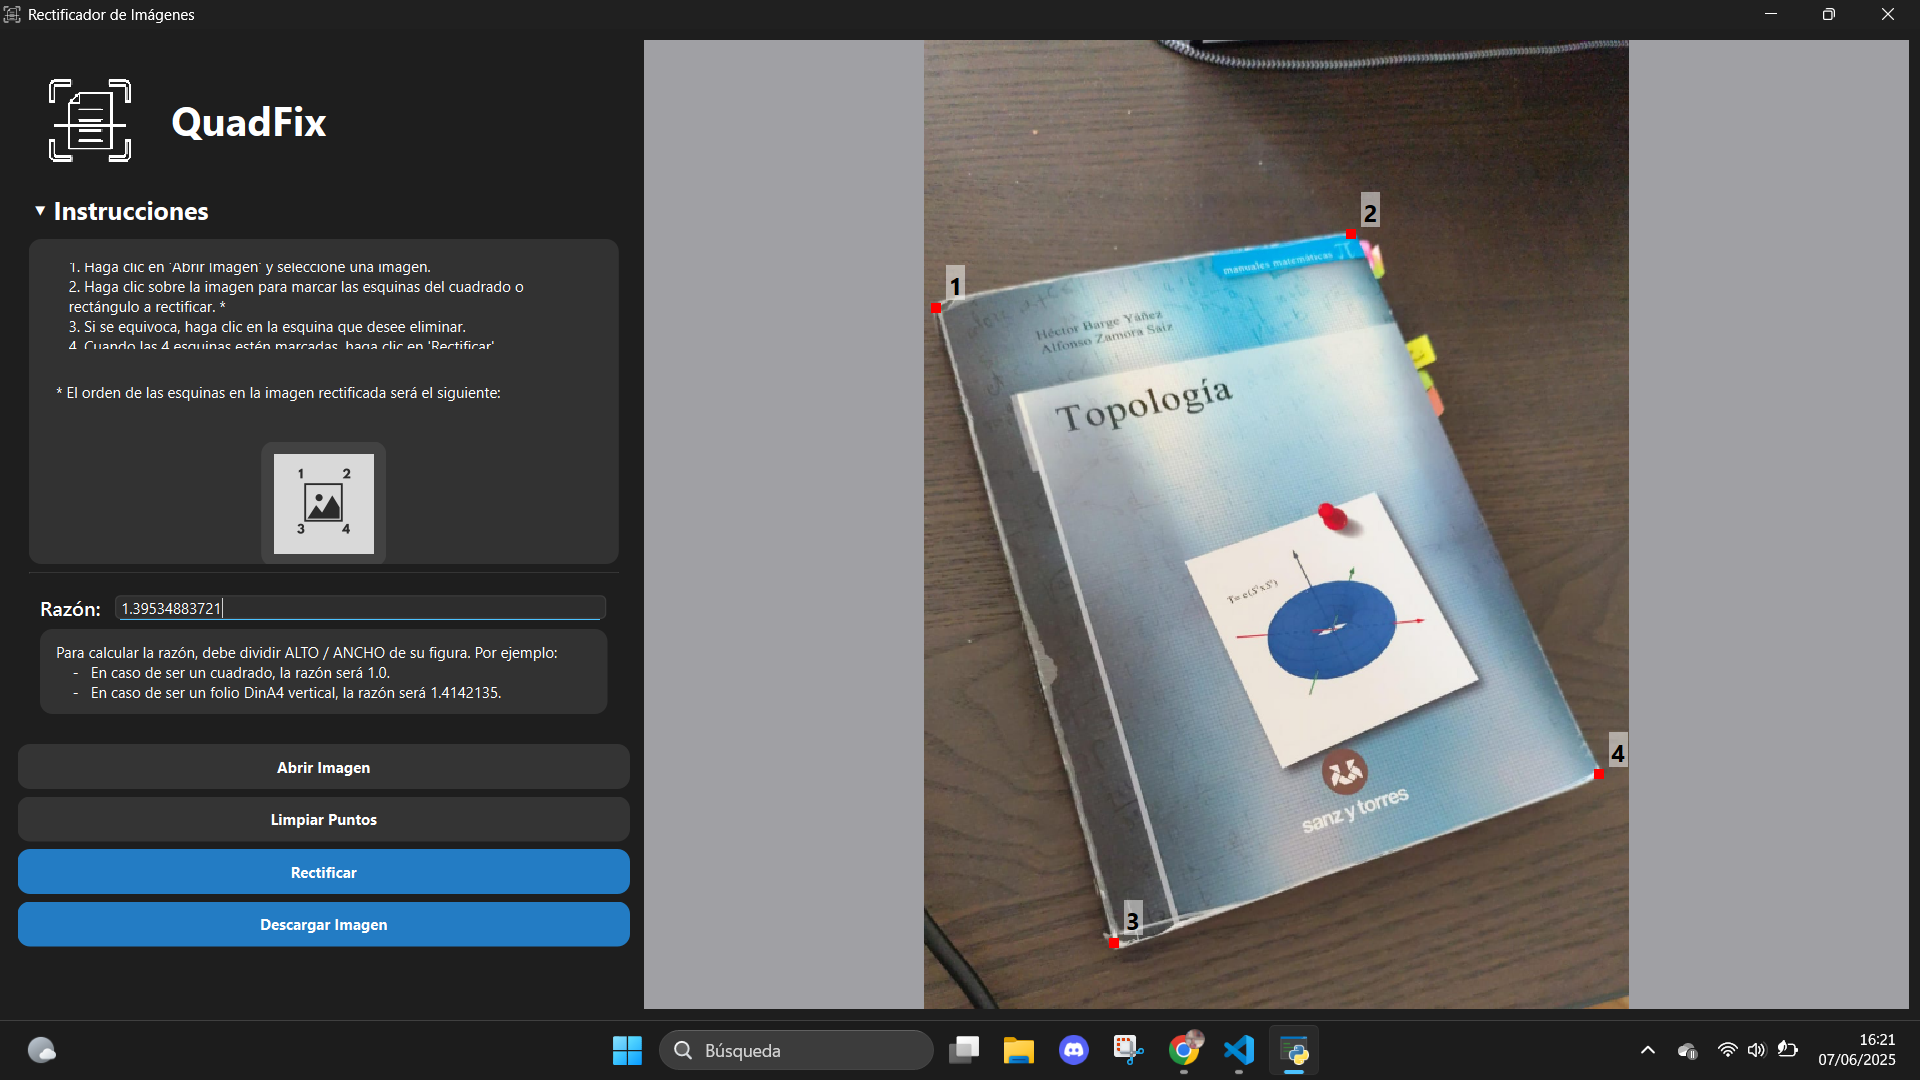
\includegraphics[width=0.85\textwidth]{figures/4.Examples/Especial/Libro1.png}
    \caption{Libro con proporción 1.395: imagen original con esquinas marcadas}
    \label{fg:libro-original}
\end{figure}

La Figura~\ref{fg:libro-rectificado} muestra el resultado tras la aplicación de la homografía y el escalado anisotrópico. La portada ha sido rectificada correctamente, conservando sus proporciones reales.

\begin{figure}[H]
    \centering
    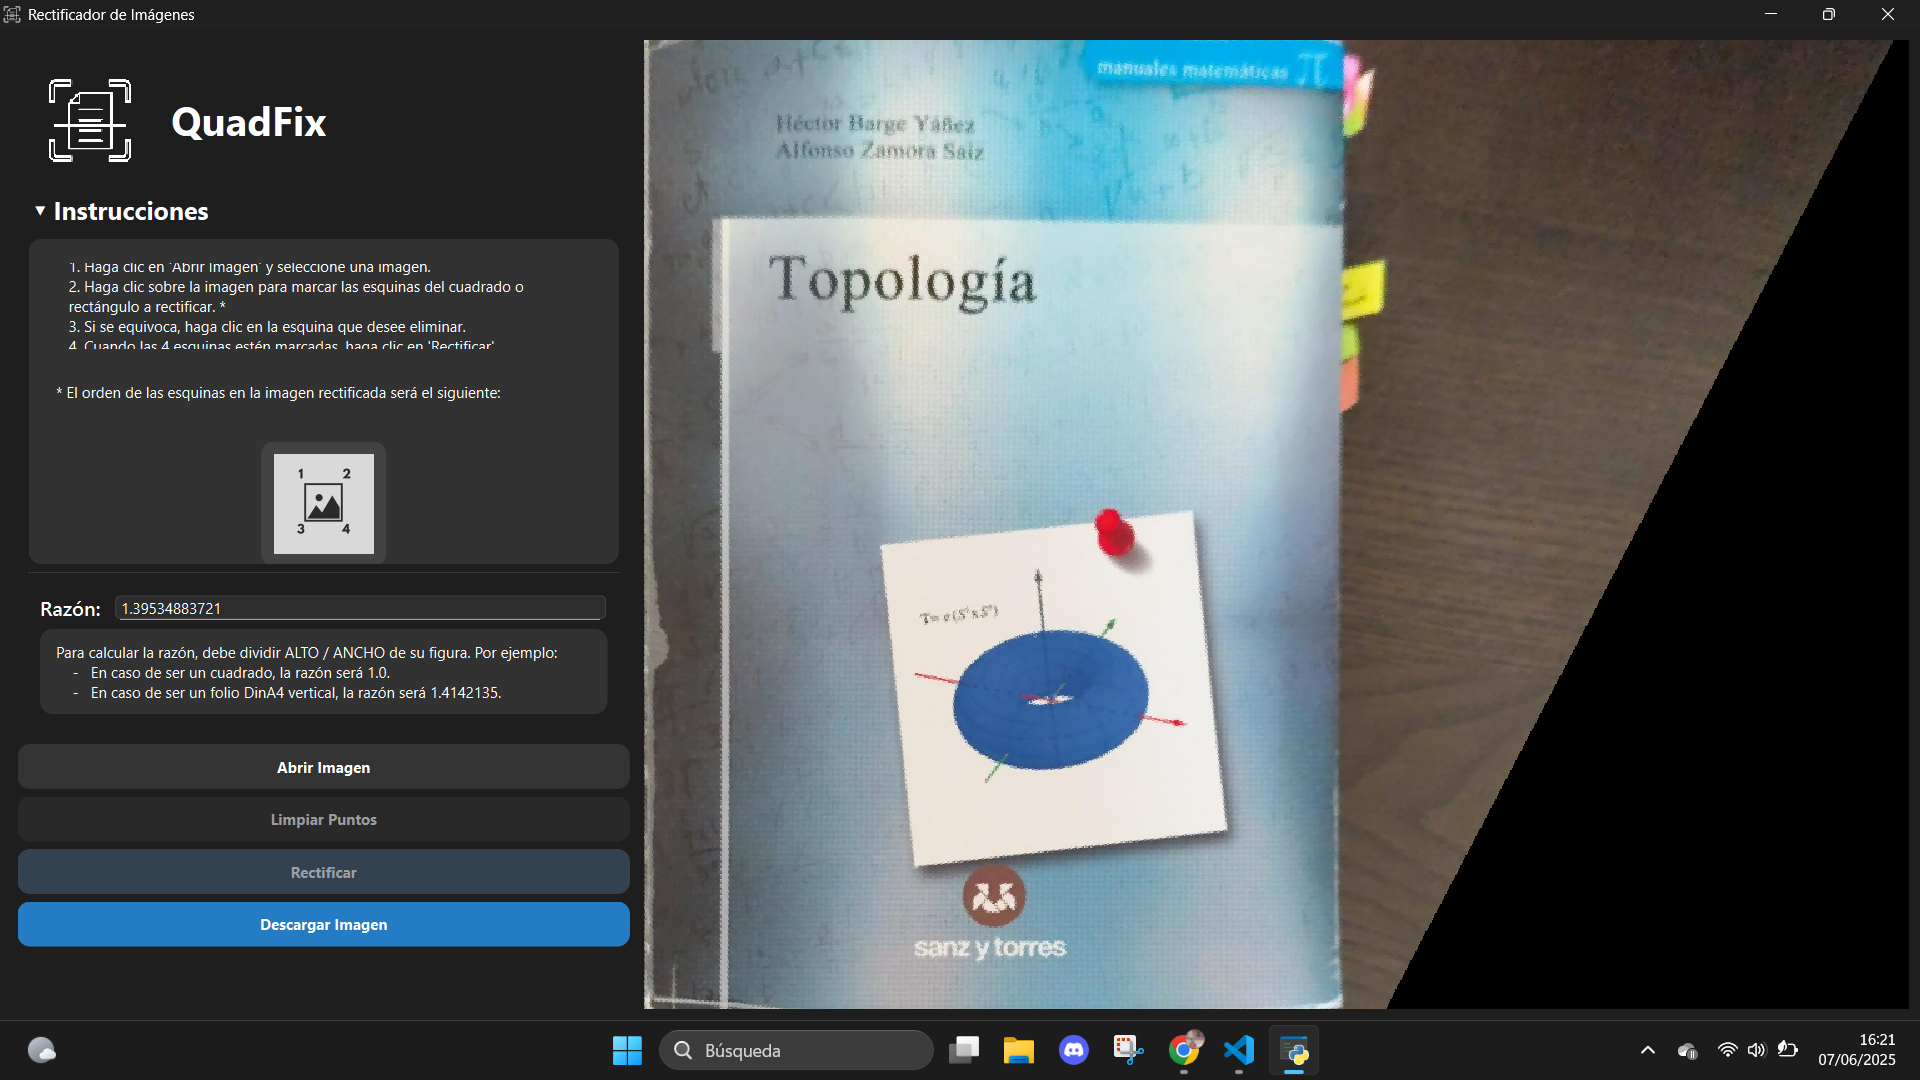
\includegraphics[width=0.85\textwidth]{figures/4.Examples/Especial/Libro2.png}
    \caption{Resultado de la rectificación del libro}
    \label{fg:libro-rectificado}
\end{figure}

\subsubsection*{Ejemplo 2: Cuadro con orientación horizontal}

Este segundo caso ilustra un problema común cuando se rectifican objetos cuya anchura es mayor que su altura. El cuadro en cuestión tiene dimensiones de $101$ cm de ancho por $70.5$ cm de alto. Según las instrucciones de la aplicación, lo más intuitivo sería introducir la razón como $ALTO/ANCHO = 70.5 / 101 = 0.698$, y seleccionar las esquinas siguiendo el orden indicado.

La Figura~\ref{fg:cuadro-invalido-1} muestra la imagen en la interfaz con la razón introducida y las esquinas marcadas según ese criterio. La Figura~\ref{fg:cuadro-invalido-2} muestra el resultado incorrecto, en el que puede observarse una distorsión visual significativa. Este tipo de error se explica en la Sección~\ref{sec:limitaciones}, donde se abordan los problemas relacionados con el manejo de errores.

\begin{figure}[H]
    \centering
    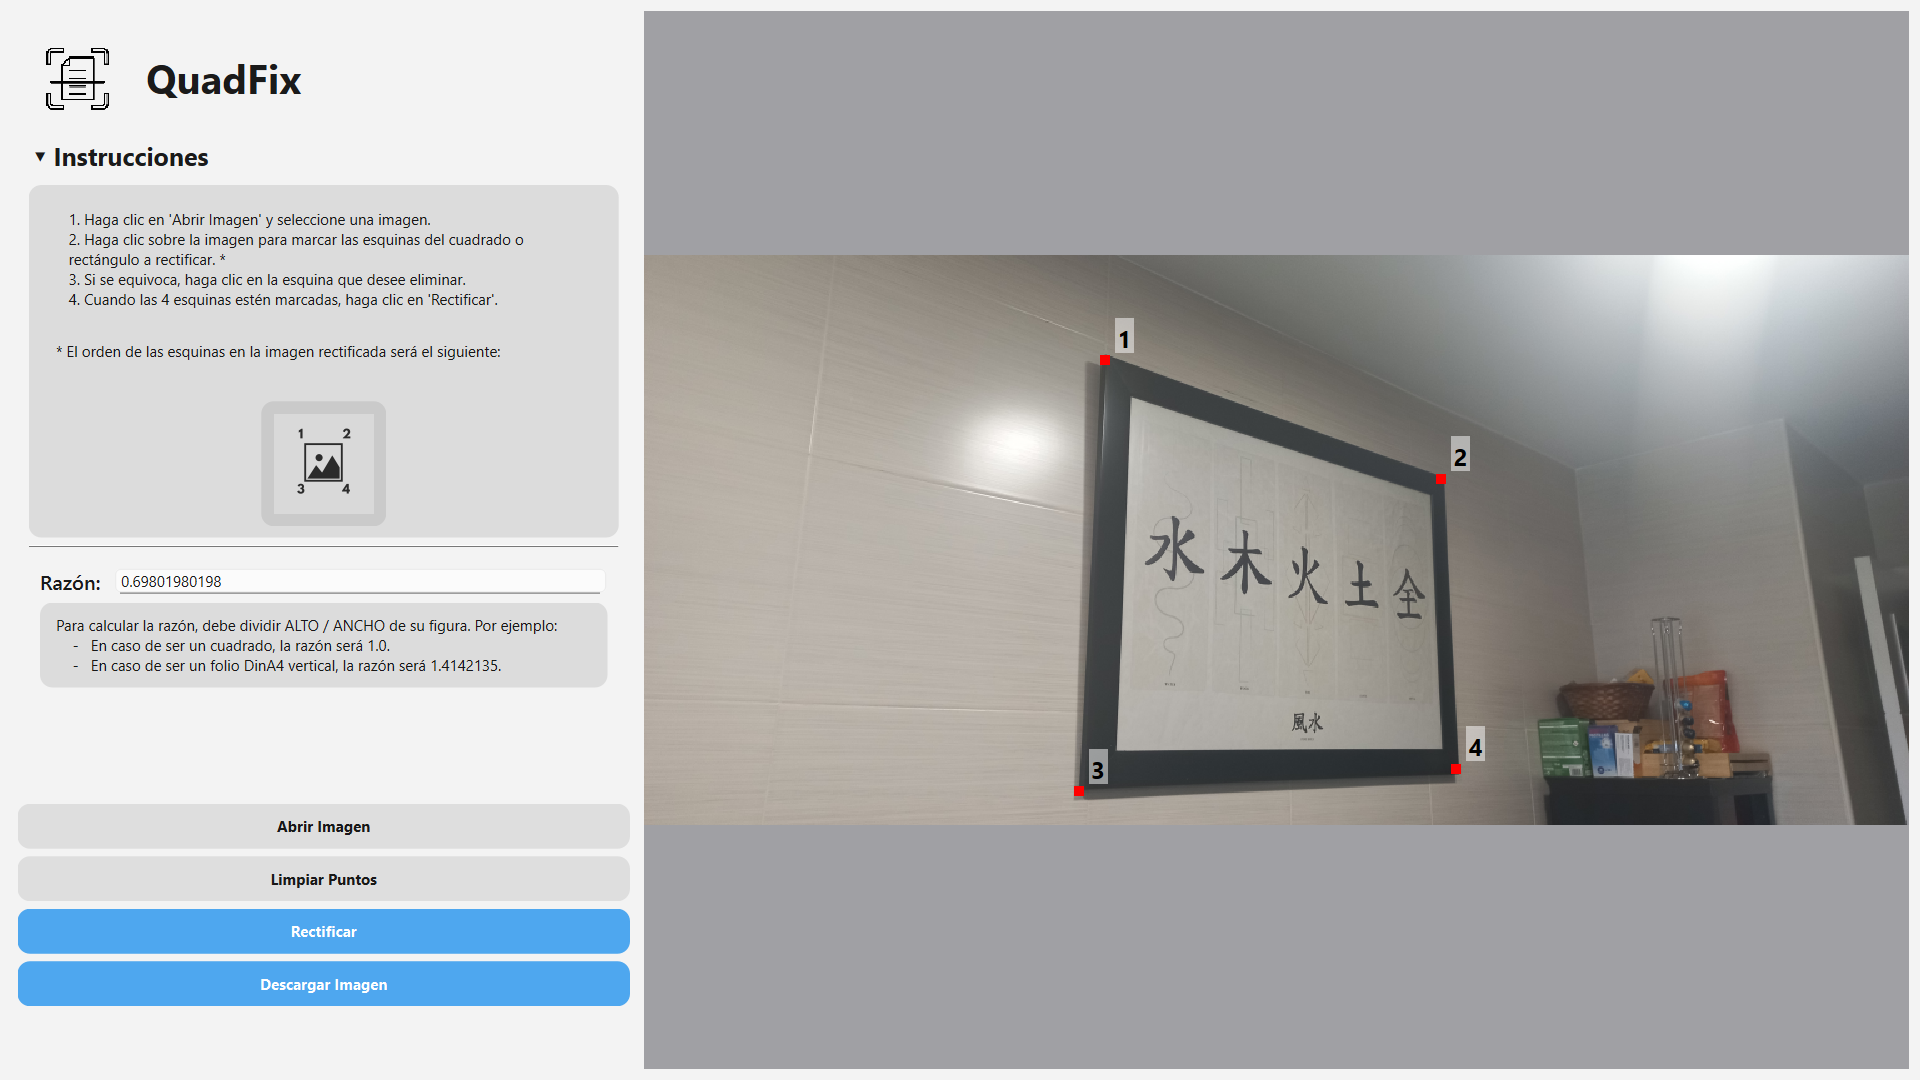
\includegraphics[width=0.6\textwidth]{figures/4.Examples/Especial/CuadroError1.png}
    \caption{Cuadro con razón 0.698 y esquinas seleccionadas en orden estándar}
    \label{fg:cuadro-invalido-1}
\end{figure}

\begin{figure}[H]
    \centering
    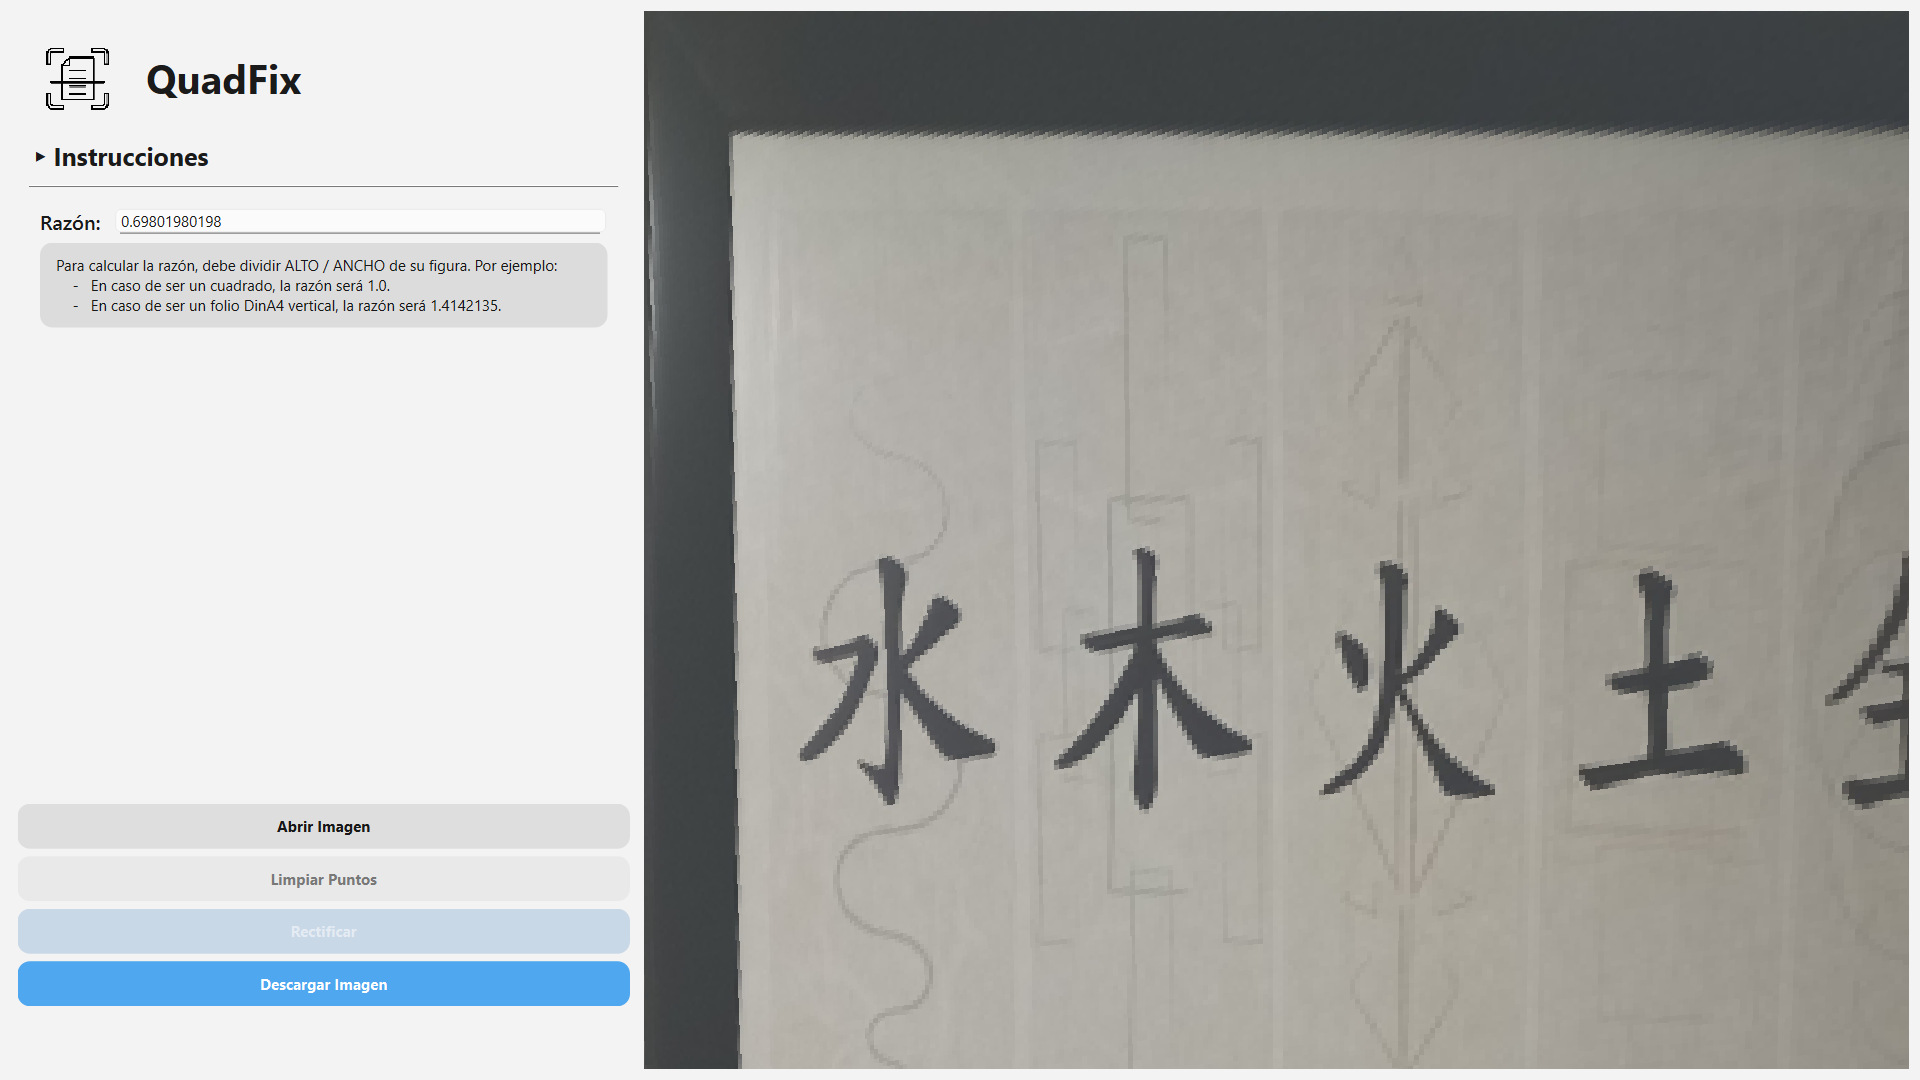
\includegraphics[width=0.6\textwidth]{figures/4.Examples/Especial/CuadroError2.png}
    \caption{Resultado erróneo de la rectificación con orientación incorrecta}
    \label{fg:cuadro-invalido-2}
\end{figure}

La solución consiste en pensar el objeto como si estuviera girado $-90^\circ$, es decir, considerar su orientación vertical. Así, la razón introducida pasa a ser $101 / 70.5 \approx 1.433$, y el orden de selección de las esquinas también se modifica. El resultado aparece girado, pero la rectificación es correcta y proporcional, como puede verse en las Figuras~\ref{fg:cuadro-corregido-1} y \ref{fg:cuadro-corregido-2}.

\begin{figure}[H]
    \centering
    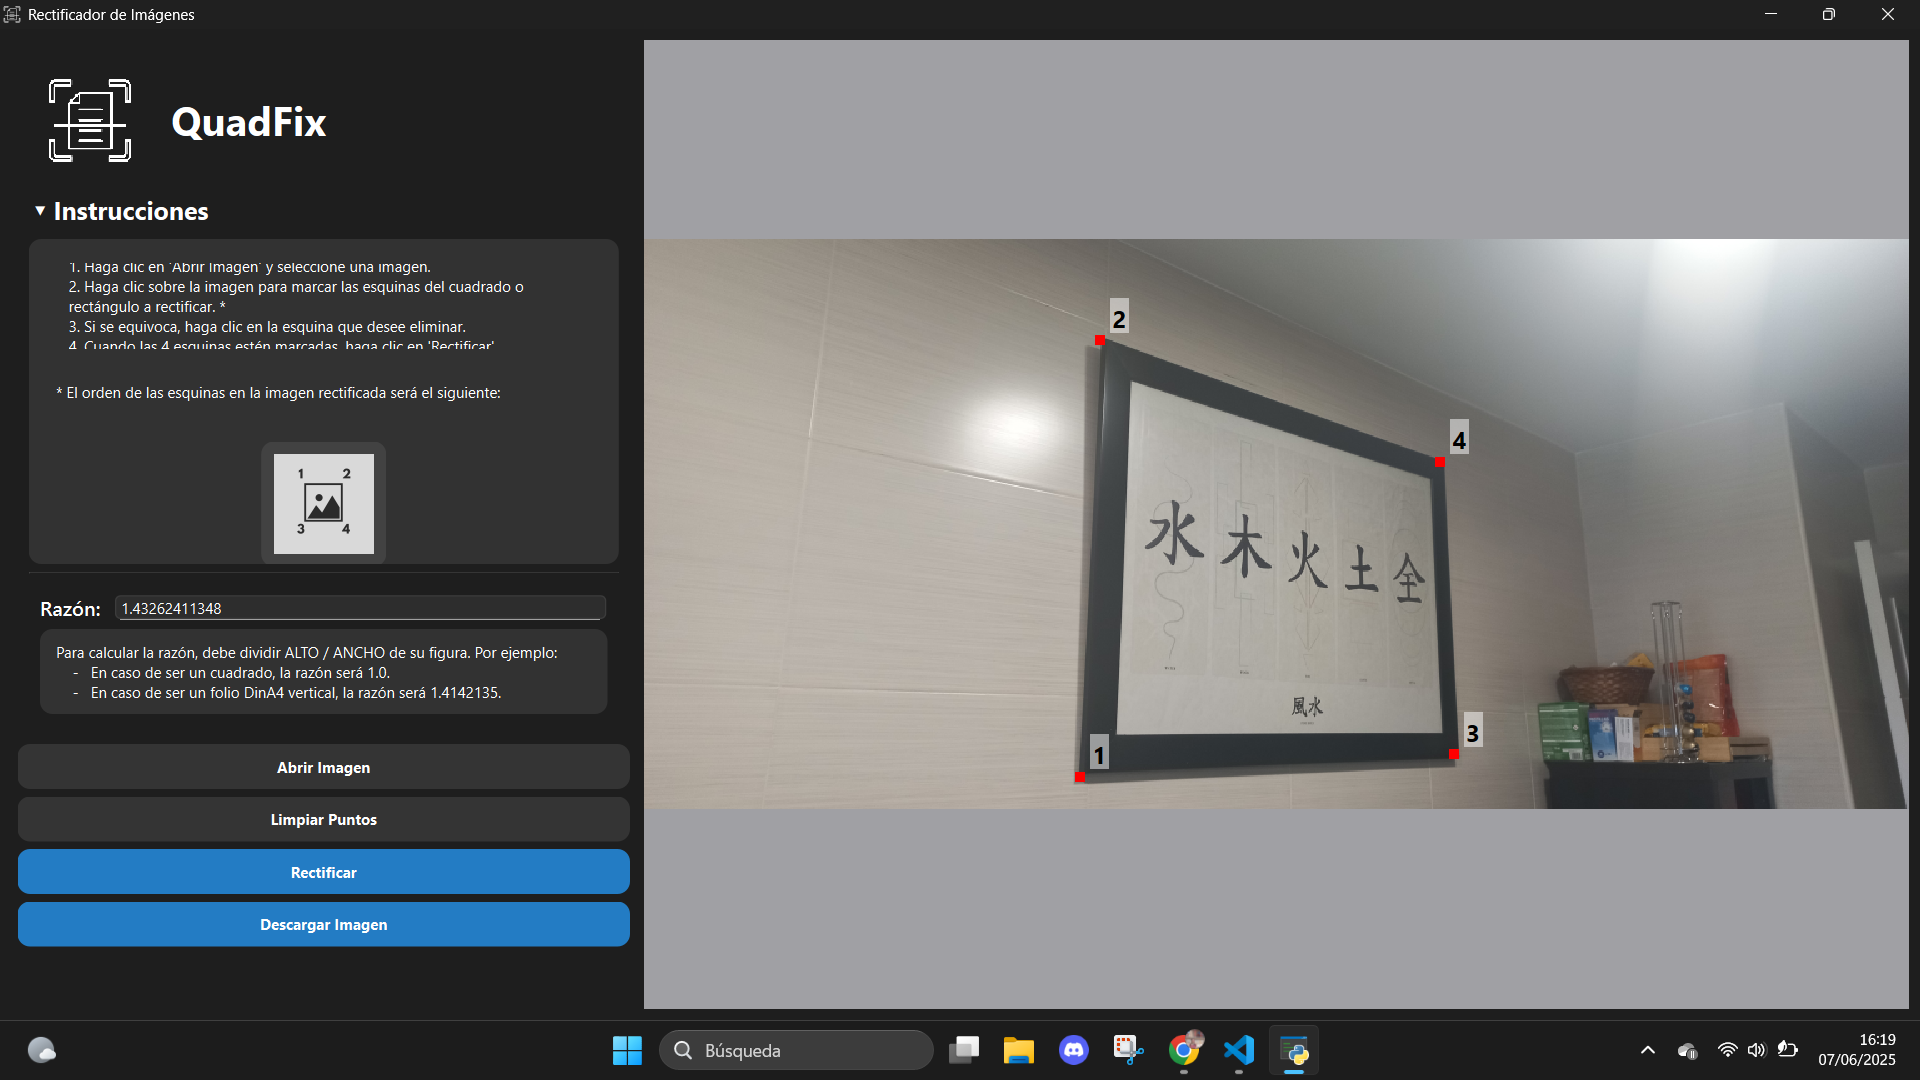
\includegraphics[width=0.6\textwidth]{figures/4.Examples/Especial/Cuadro1.png}
    \caption{Cuadro tratado como imagen vertical: razón $1.433$ y nuevo orden de esquinas}
    \label{fg:cuadro-corregido-1}
\end{figure}

\begin{figure}[H]
    \centering
    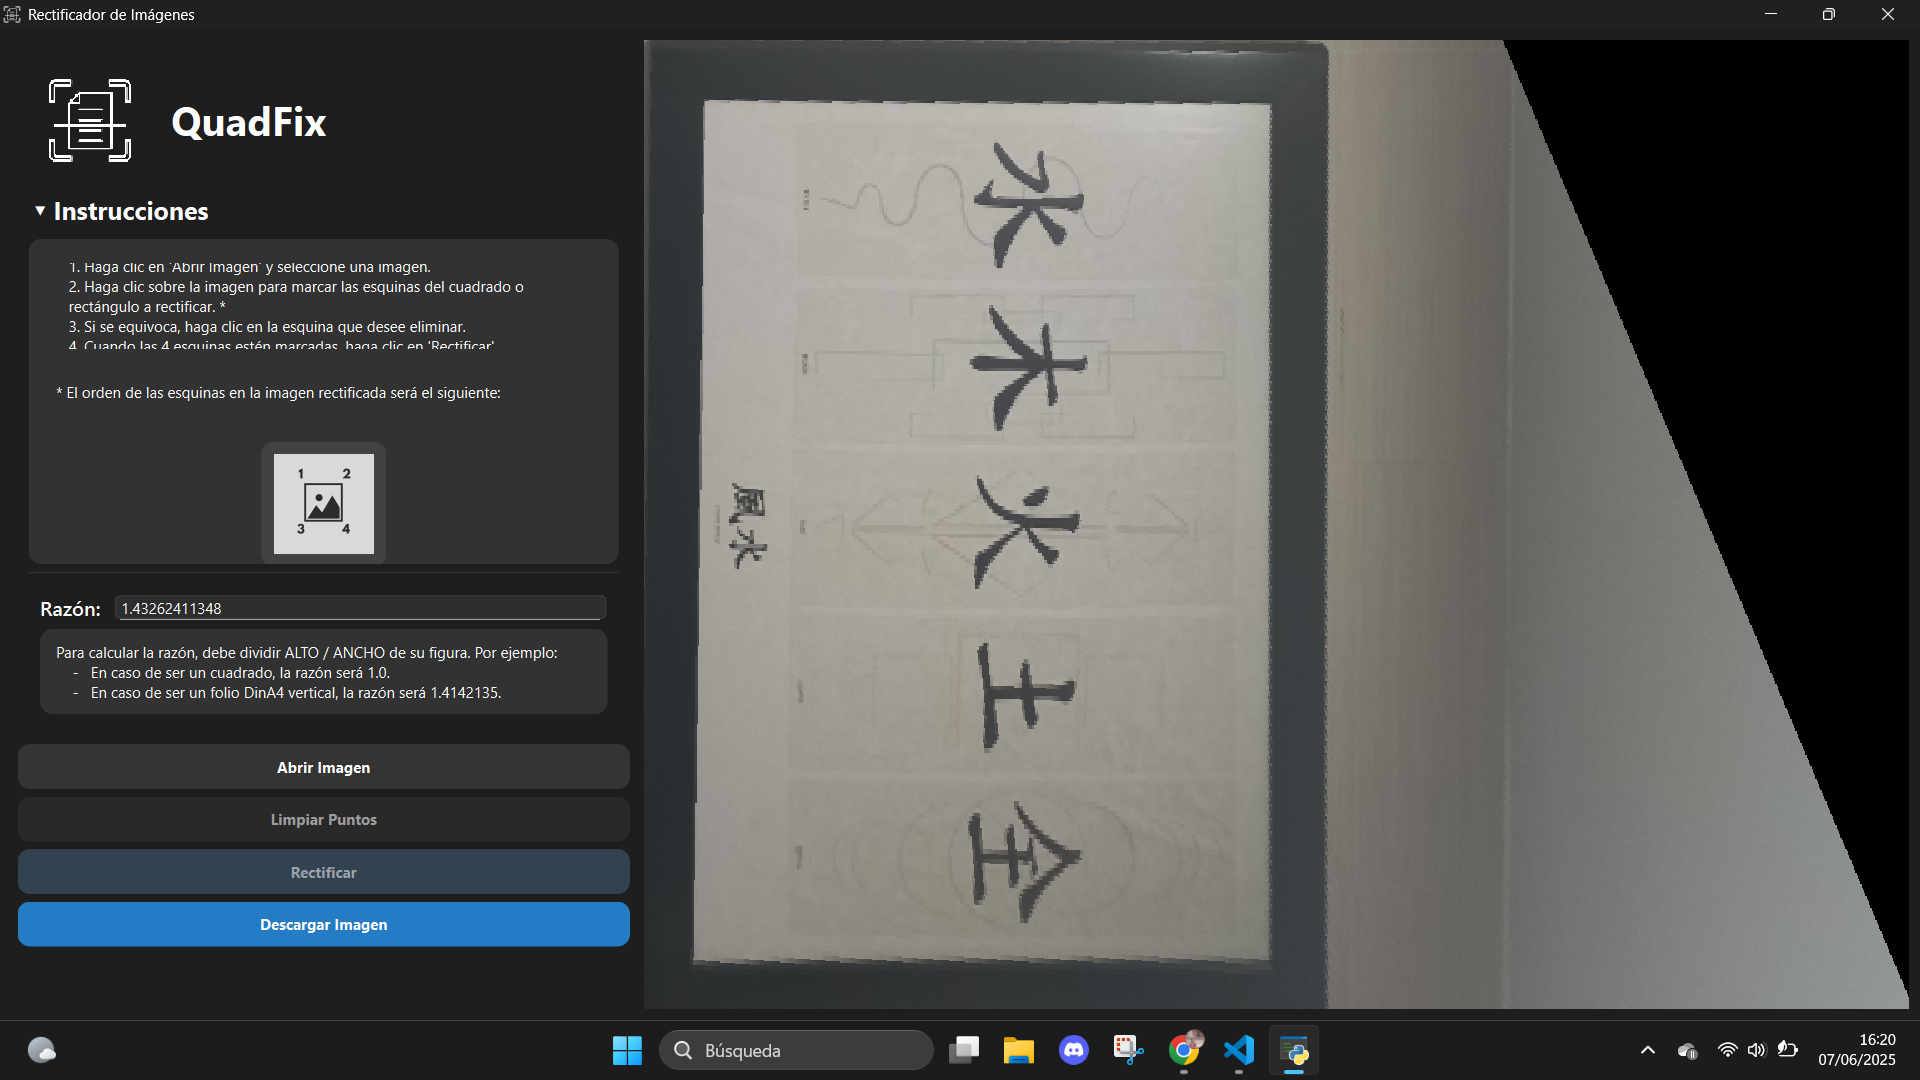
\includegraphics[width=0.6\textwidth]{figures/4.Examples/Especial/Cuadro2.png}
    \caption{Resultado correcto tras interpretar la imagen con rotación $-90^\circ$}
    \label{fg:cuadro-corregido-2}
\end{figure}
